\documentclass[10pt]{beamer}

\usetheme[subsectionpage=progressbar]{metropolis}
\usepackage{appendixnumberbeamer}

\usepackage{ucs}
\usepackage[utf8x]{inputenc}
\usepackage[ngerman]{babel}

\usepackage{booktabs}
\usepackage[scale=2]{ccicons}

\usepackage{pgfplots}
\usepgfplotslibrary{dateplot}

\usepackage{xspace}
\usepackage{dsfont}
\usepackage{graphicx}
\newcommand{\themename}{\textbf{\textsc{metropolis}}\xspace}

\title{Nummernschilderkennung mit Python}
% \subtitle{Machine Learning in Produktion und Logistik}
\date{19. Januar 2021}
\author{Anne-Sophie Bollmann, Susanne Kl\"ocker, Pia von Kolken, Christian Peters}
%\institute{TU Dortmund}
%\titlegraphic{\hfill\includegraphics[height=1.5cm]{logo.pdf}}

\begin{document}

\maketitle

\begin{frame}{Inhalt}
  \setbeamertemplate{section in toc}[sections numbered]
  \tableofcontents
\end{frame}

\section{Einleitung}

\begin{frame}{Einleitung}
    Hier kommt irgendwas fffff hin.
\end{frame}

\begin{frame}{Ein Titel}
    Hier kann man einfach was hinschreiben.
    Aufz\"ahlungen gehen nat\"urlich auch:
    \begin{itemize}
        \item Dies
        \item und
        \item das
    \end{itemize}
\end{frame}

\section{Extraktion des Nummernschildes}

\begin{frame}{Convolutional Neural Networks}
    \begin{figure}
        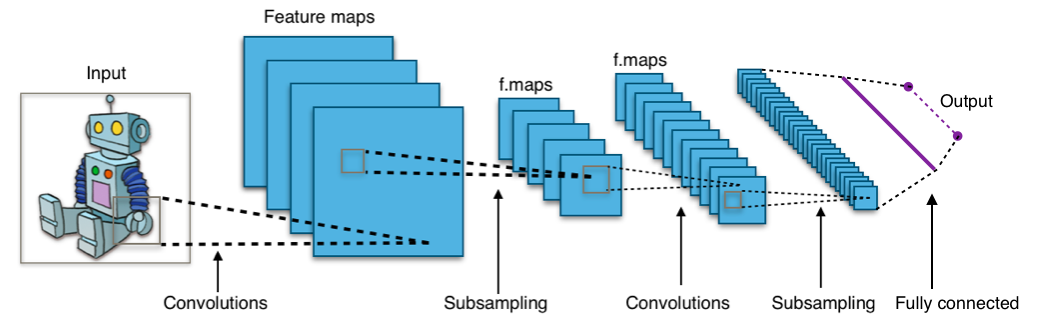
\includegraphics[width=\textwidth]{bilder/Typical_cnn.png}
        \caption{Convolutional Neural Network.
            \footnote{Bildquelle: \url{https://de.wikipedia.org/wiki/Convolutional_Neural_Network}}}
    \end{figure}
    \begin{center}
        \fbox{\textbf{Input:} Bild mit Auto $\longmapsto$ \textbf{Output:} Bounding Box}
    \end{center}
\end{frame}

\begin{frame}{Implementierung mit Keras}
    \begin{itemize}
        \item TODO
    \end{itemize}
\end{frame}

\section{Nummernschild auslesen}

\begin{frame}{Nummernschild auslesen}

Wie können wir Text auf Bildern auslesen?

\begin{itemize}
\item Tesseract: freie Software zur Texterkennung mit vielen vorimplementierten Sprachen \cite{smith_2007}
\item Problem: Text wird größtenteils noch nicht richtig auf den unbearbeiteten Nummernschildern erkannt
\item Lösung: das erkannte Nummernschild derart vorverarbeiten (preprocessing), dass das richtige Auslesen der einzelnen Elemente möglichst gut unterstützt wird
\end{itemize}

\end{frame}

\begin{frame}{Nummernschild vorverarbeiten}

\begin{itemize}
\item Geeignetes Werkzeug: OpenCV \cite{opencv_tutorial}
\item OpenCV ist eine plattformübergreifende Bibliothek, für Echtzeit-Computer-Vision-Anwendungen
\item beinhaltet Algorithmen für die Bildverarbeitung und im Rahmen von Computer Vision (CV) auch für maschinelles Lernen
\item Nutzung für die Verarbeitung des erkannten Nummernschildes (z.B. Thresholding), um die Zeichen besser zu erkennen und richtig auszulesen
\end{itemize}

\end{frame}

\begin{frame}{Beispiel für die Anwendung von OpenCV}

OpenCV wurde bereits auf Nummernschildverarbeitung verwendet:
\begin{figure}
\begin{center}
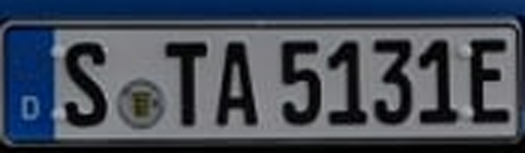
\includegraphics[scale=0.25]{bilder/Nummer_1.png}
\caption{Original
\footnote{Bildquelle: \url{https://github.com/theAIGuysCode/yolov4-custom-functions}}}
\label{Original}
\end{center}
\end{figure}

\begin{figure}
\begin{center}
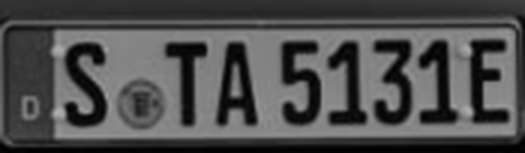
\includegraphics[scale=0.25]{bilder/Nummer_2_grau.png}
\caption{Graustufen}
\label{Graustufen}
\end{center}
\end{figure}

\end{frame}

\begin{frame}{Beispiel für die Anwendung von OpenCV}

\begin{figure}
\begin{center}

\includegraphics[scale=0.25]{bilder/Nummer_3_treshold.png}
\caption{Thresholding}
\label{Tresholding}
\end{center}
\end{figure}

\begin{figure}
\begin{center}
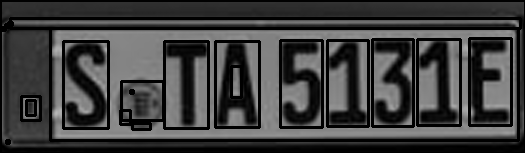
\includegraphics[scale=0.25]{bilder/Nummer_4_Konturen.png}
\caption{Konturen}
\label{Konturen}
\end{center}
\end{figure}

\end{frame}

\begin{frame}{Beispiel für die Anwendung von OpenCV}

\begin{figure}
\begin{center}
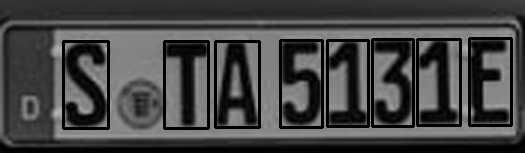
\includegraphics[scale=0.25]{bilder/Nummer_5_Aussortieren.png}
\caption{Aussortierung}
\label{Aussortierung}
\end{center}
\end{figure}

\begin{figure}
\begin{center}

\includegraphics[scale=0.25]{bilder/Nummer_6_SchwarzWeiss.png}
\caption{Schwarze Schrift auf weißem Hintergrund}
\label{SchwarzWeiss}
\end{center}
\end{figure}

Auf das finale Bild (Abbildung \ref{Aussortierung}) wird anschließend Tesseract angewendet, das die Nummern und Buchstaben ausgibt
\end{frame}

\begin{frame}{Validierung der Texterkennung}
    \textbf{Validierung:}
    \begin{itemize}
    \item Rastersuche über Parametereinstellungen für OpenCV
    \item Validierung über \textit{character accuracy} \cite{ocr_accuracy}:
    \begin{align*}
    \frac{n - \# \textit{errors}}{n},
    \end{align*}
    wobei $n$ Anzahl der Zeichen im Datensatz und $\# \textit{errors}$ Anzahl der fehlerhaft erkannten Zeichen 
    \item[$\rightarrow$] Parametereinstellungen mit höchstem \textit{character accuracy} werden für Texterkennung verwendet
    \end{itemize}
\end{frame}

\section{Tesseract}

\begin{frame}{Tesseract}
    \begin{itemize}
    	\item freie Software zur Texterkennung 
    	\item häufig erprobt für eine Vielzahl von Problemen 
    	% License Plate, Handschrift, Frakturtexte, ...
    \end{itemize}
    \vspace{0.2cm}
    \begin{itemize}
    	\item hier Bild hin?
    \end{itemize}
\end{frame}

\begin{frame}[standout]
  Irgendwas zum Schluss
\end{frame}

\appendix

\begin{frame}[allowframebreaks]{Literatur}

  \bibliography{literatur}
  \bibliographystyle{abbrv}

\end{frame}

\end{document}
